\documentclass[aspectratio=169]{beamer}
%
% Choose how your presentation looks.
%
% For more themes, color themes and font themes, see:
% http://deic.uab.es/~iblanes/beamer_gallery/index_by_theme.html
%
\mode<presentation>
{
    \usetheme{default}      % or try Darmstadt, Madrid, Warsaw, ...
    \usecolortheme{default} % or try albatross, beaver, crane, ...
    \usefonttheme{default}  % or try serif, structurebold, ...
    \setbeamertemplate{navigation symbols}{}
    \setbeamertemplate{caption}[numbered]
}

\usepackage[english]{babel}
\usepackage[utf8]{inputenc}
\usepackage{graphicx}
\usepackage{breqn}
\usepackage{bbm}

\newenvironment{wideitemize}{\itemize\addtolength{\itemsep}{10pt}}{\enditemize}
\newenvironment{transitionframe}{
    \setbeamercolor{background canvas}{bg=white}
    \begin{frame}}{
    \end{frame}
}

\DeclareMathOperator*{\argmax}{arg\,max}
\DeclareMathOperator*{\argmin}{arg\,min}

\usepackage[style=authoryear, backend=biber]{biblatex}
\addbibresource{econ281_presentation.bib}

\title{Flatter experience-wage profiles and declining labor force nonparticipation}
\author{Churn Ken Lee}
\institute{UC San Diego}
\date{}

\begin{document}

\frame{\titlepage}

\begin{frame}
    \frametitle{Motivation}

    Declining labor force participation among prime-aged low-skilled men (Binder \& Bound JEP 2019)
    \begin{figure}[t]
        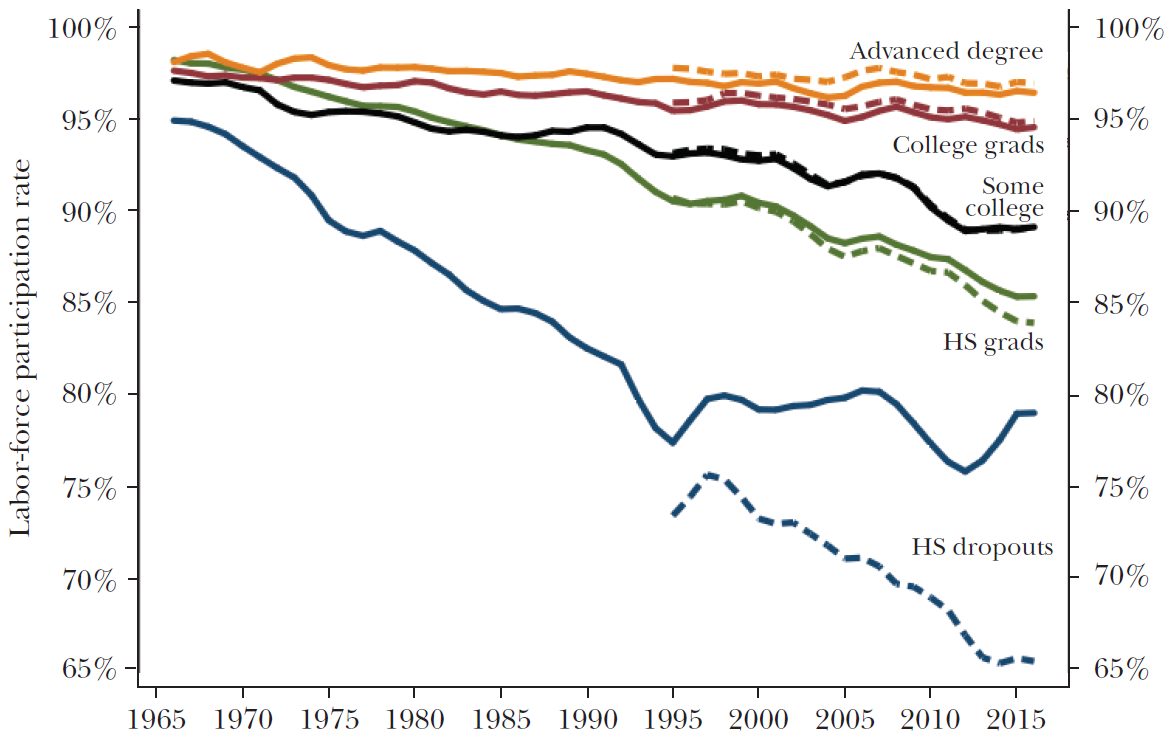
\includegraphics[width=0.7\textwidth]{../output/participation_education.png}
        \centering
    \end{figure}

\end{frame}

\begin{frame}
    \frametitle{Motivation}

    Flattening of experience-income profile of low-skilled relative to high-skilled (Elsby \& Shapiro AER 2012)
    \begin{figure}[t]
        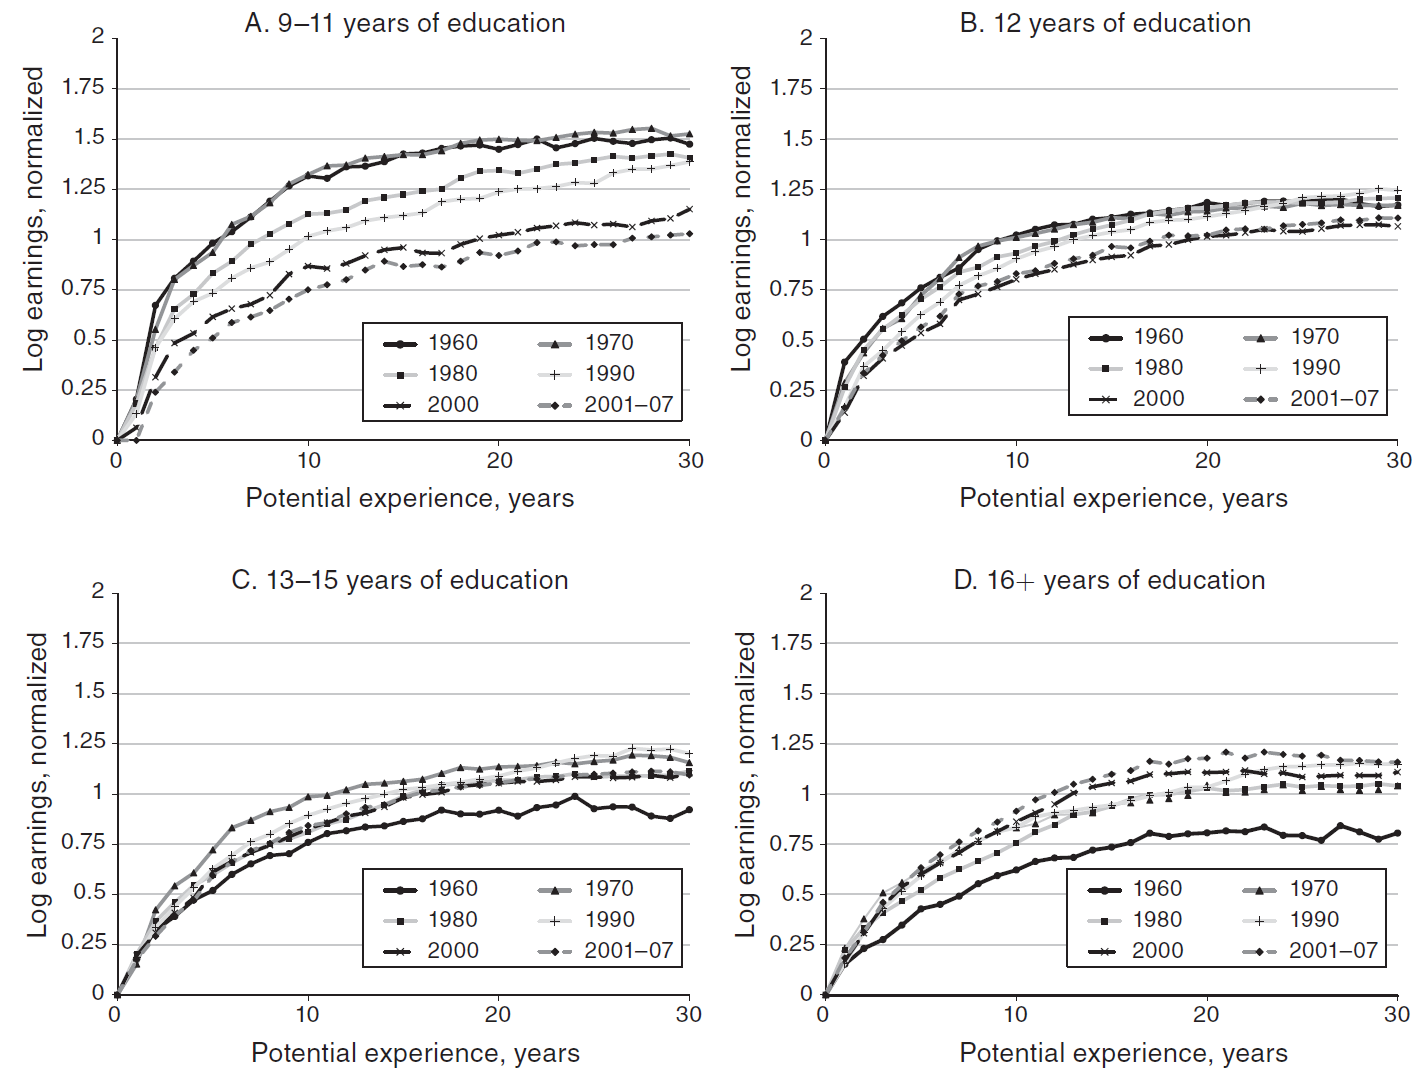
\includegraphics[width=0.65\textwidth]{../output/profile_cross_elsby_shapiro.png}
        \centering
    \end{figure}
\end{frame}

\begin{frame}
    \frametitle{Motivation}

    Flattening of experience-income profile of low-skilled relative to high-skilled (Elsby \& Shapiro AER 2012)
    \begin{figure}[t]
        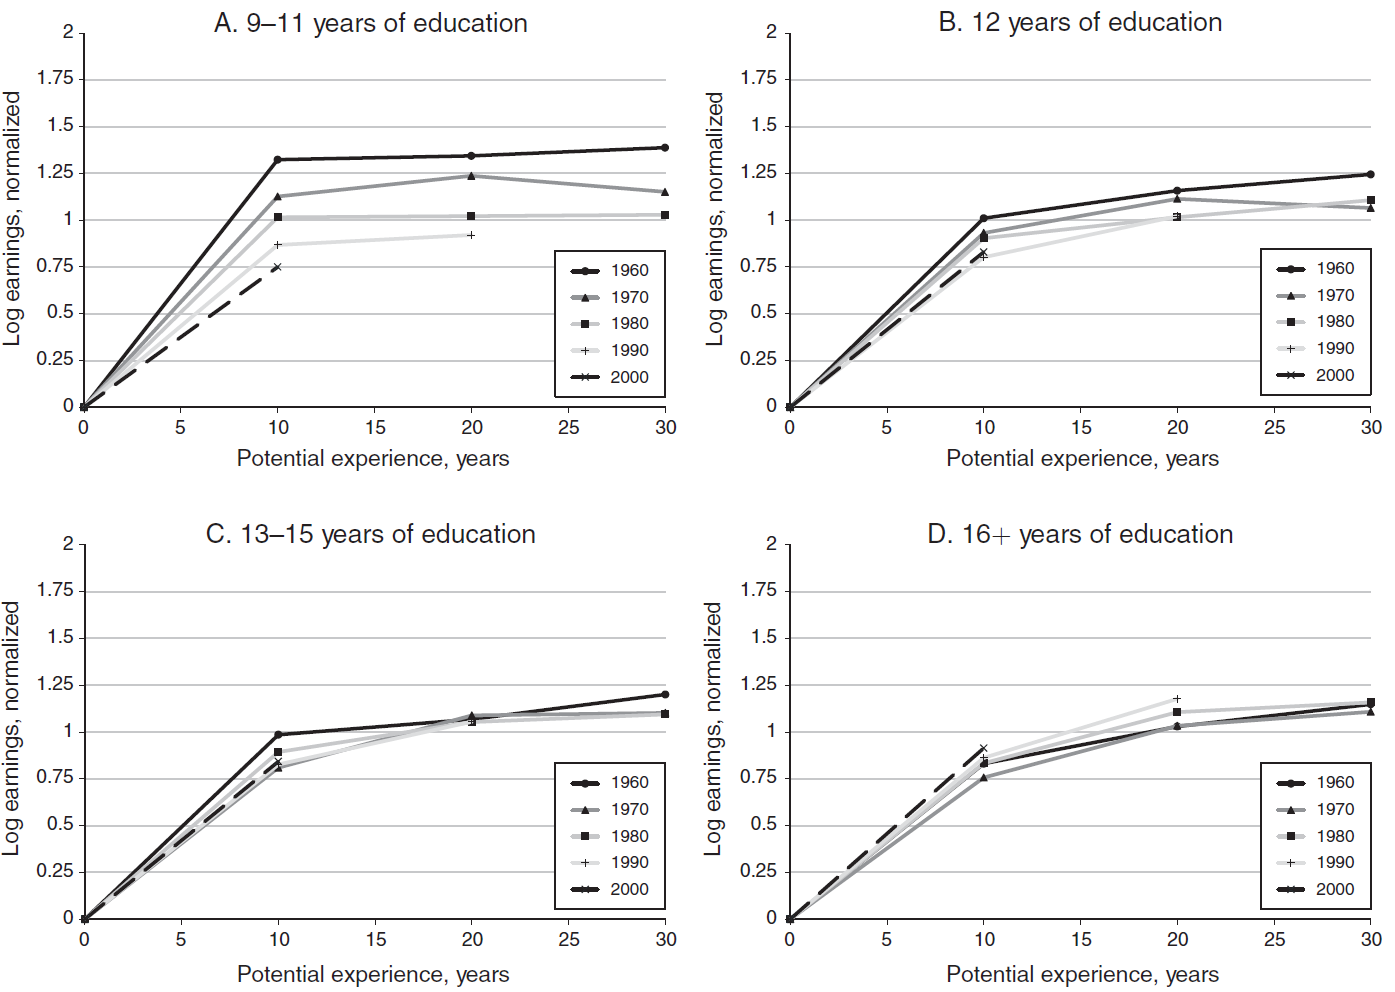
\includegraphics[width=0.65\textwidth]{../output/profile_cohort_elsby_shapiro.png}
        \centering
    \end{figure}

\end{frame}

\begin{frame}
    \frametitle{Motivation}

    Experience-income profile of lowest-skilled has actually steepened recently!
    \begin{figure}[t]
        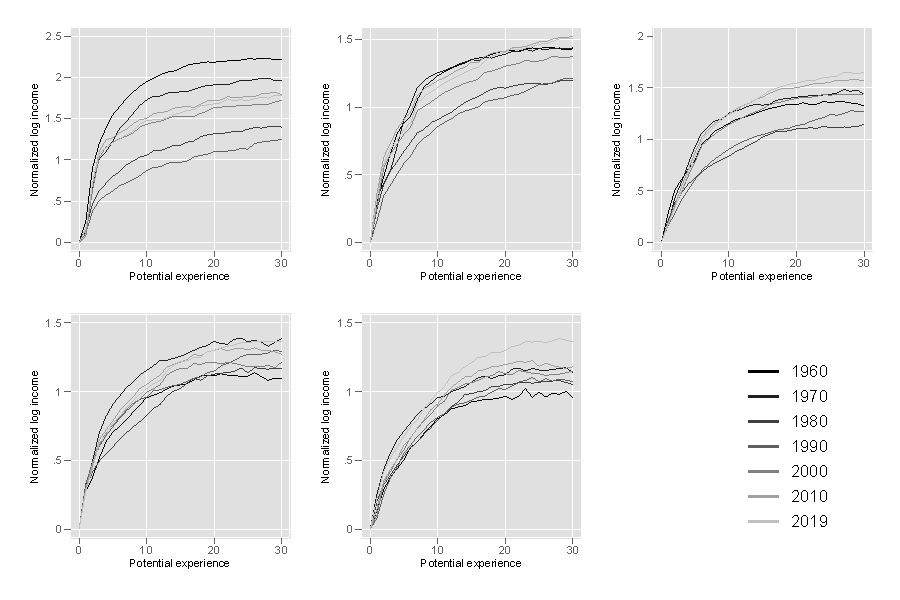
\includegraphics[width=0.8\textwidth]{../output/exp_wage_profile_cross.pdf}
        \centering
    \end{figure}
\end{frame}

\begin{frame}
    \frametitle{Motivation}

    Experience-income profile of lowest-skilled has actually steepened recently!
    \begin{figure}[t]
        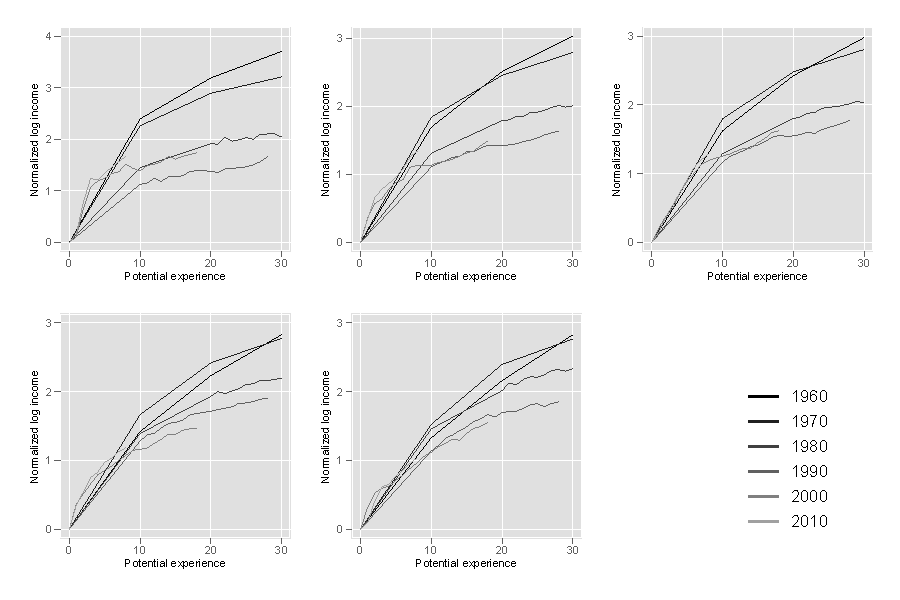
\includegraphics[width=0.8\textwidth]{../output/exp_wage_profile_cohort.pdf}
        \centering
    \end{figure}
\end{frame}

\begin{frame}
    \frametitle{Motivation}

    Increase in gap of retirement age between high and low-skilled (Rutledge 2018)
    \begin{figure}[t]
        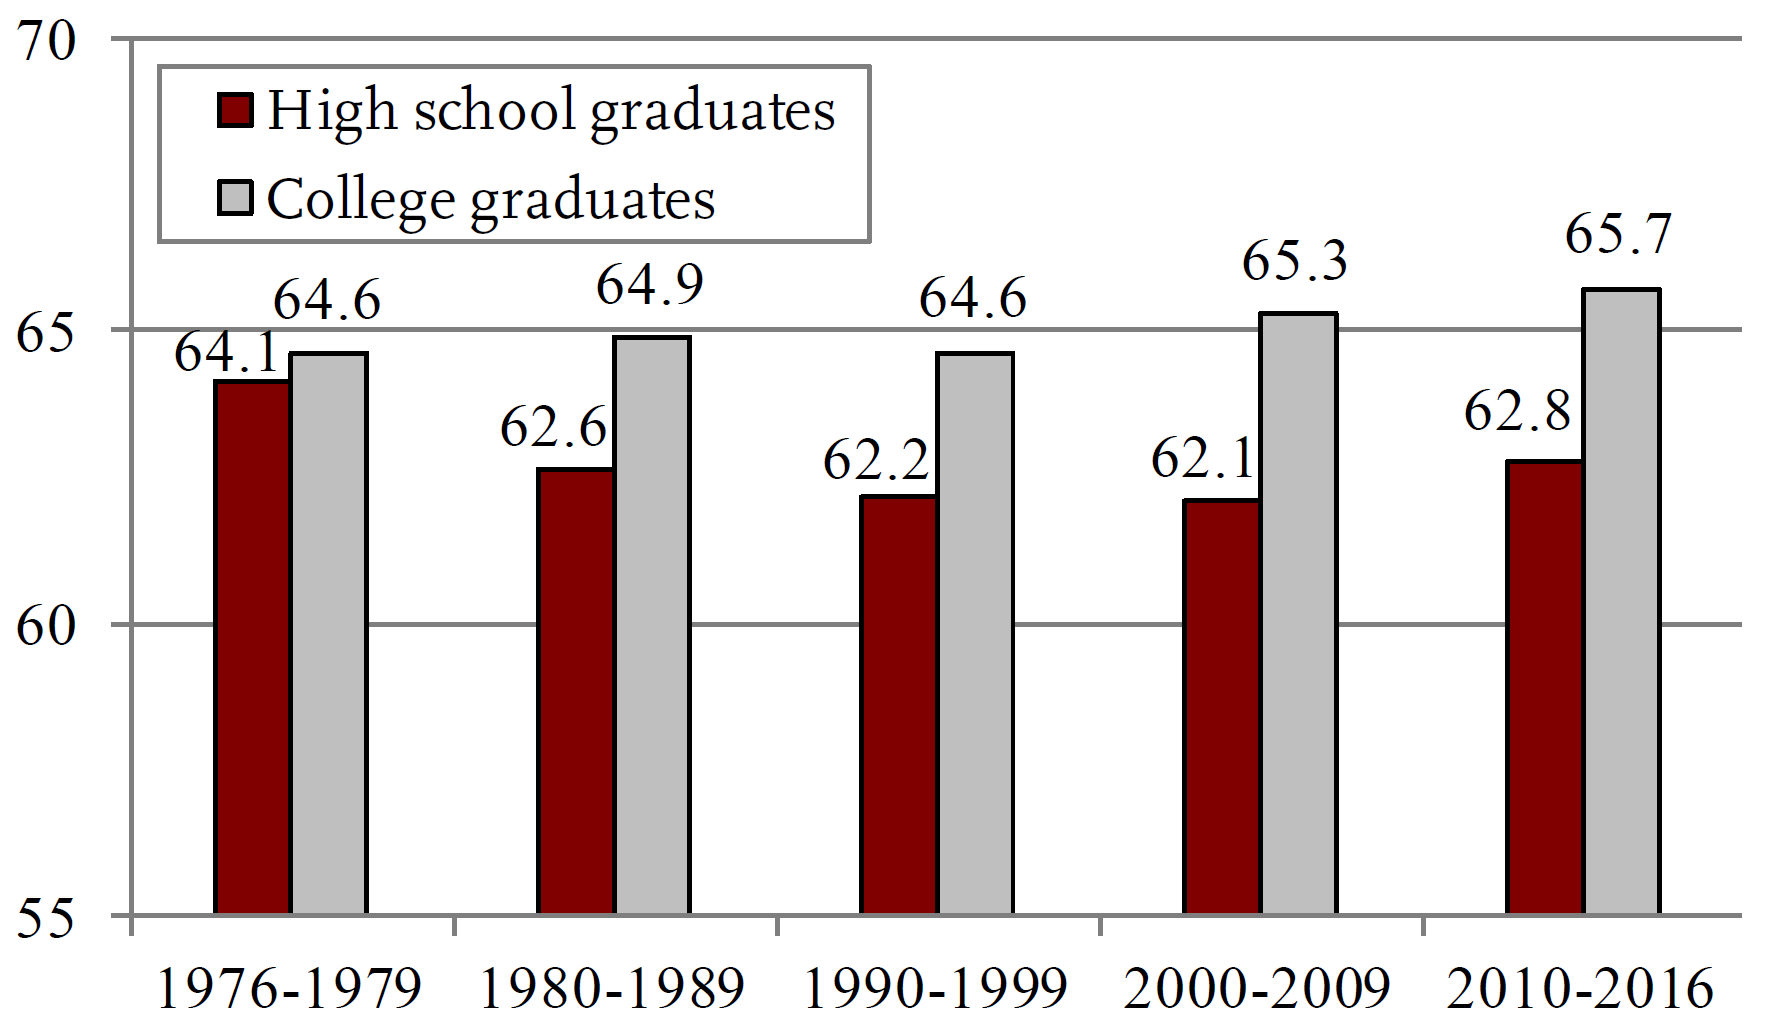
\includegraphics[width=0.8\textwidth]{../output/retirement.png}
        \centering
    \end{figure}

\end{frame}


\begin{frame}
    \frametitle{Idea}
    Declining returns to accumulation of human capital leads to
    \begin{wideitemize}
        \item less human capital accumulation
        \item lower participation
        \item and earlier retirement
    \end{wideitemize}
    among low-skilled, and lower human capital level leads to
    \begin{wideitemize}
        \item higher sensitivity and persistence to shocks
    \end{wideitemize}

\end{frame}

\begin{frame}
    \frametitle{Literature}
    Many explanations for declining LFP of prime-aged men:
    \begin{wideitemize}
        \item Skill-biased technical change (Card \& Dinardo 2002, Acemoglu \& Autor 2010)
        \item Job polarization (Foote \& Ryan 2015)
        \item Improvements in leisure technology (Aguiar et. al. 2018)
        \item Disability and SSDI (Autor \& Duggan QJE 2003, Krueger 2017)
        \item Incarceration (Binder \& Bound JEP 2019)
    \end{wideitemize}
    

\end{frame}

\begin{frame}
    \frametitle{Elements I need in my model}

    \begin{wideitemize}
        \item Human capital accumulation
        \item Education
        \item Labor supply
        \item Retirement
    \end{wideitemize}

\end{frame}

\begin{frame}
    \frametitle{Blinder-Weiss 1976}
    Agents with finite lifespan $T$ maximize lifetime utility
    \begin{equation*}
        \max_{\{ c_t \}_{t=0}^T, \{ h_t \}_{t=0}^T, \{ x_t \}_{t=0}^T} \sum_{t=0}^{T} \beta^t u(c_t, 1-h_t) + B(A_{T+1})
    \end{equation*}
    subject to
    \begin{equation*}
        A_{t+1} = (1+r)A_{t} + h_t g(x_t)K_{t} - c_{t},
    \end{equation*}
    \begin{equation*}
        K_{t+1} = (1-\delta)K_t + x_t h_t K_t,
    \end{equation*}
    \begin{equation*}
        x_t ,h_t \in [0,1],
    \end{equation*}
    \begin{wideitemize}
        \item $x_t$ and $g(x_t)$ governs tradeoff between accumulating human capital and earnings
        \item $B$ is bequest, $A$ is assets, and $K$ is human capital
    \end{wideitemize}

\end{frame}

\begin{frame}
    \frametitle{$g(x)$}
    
    \begin{figure}[t]
        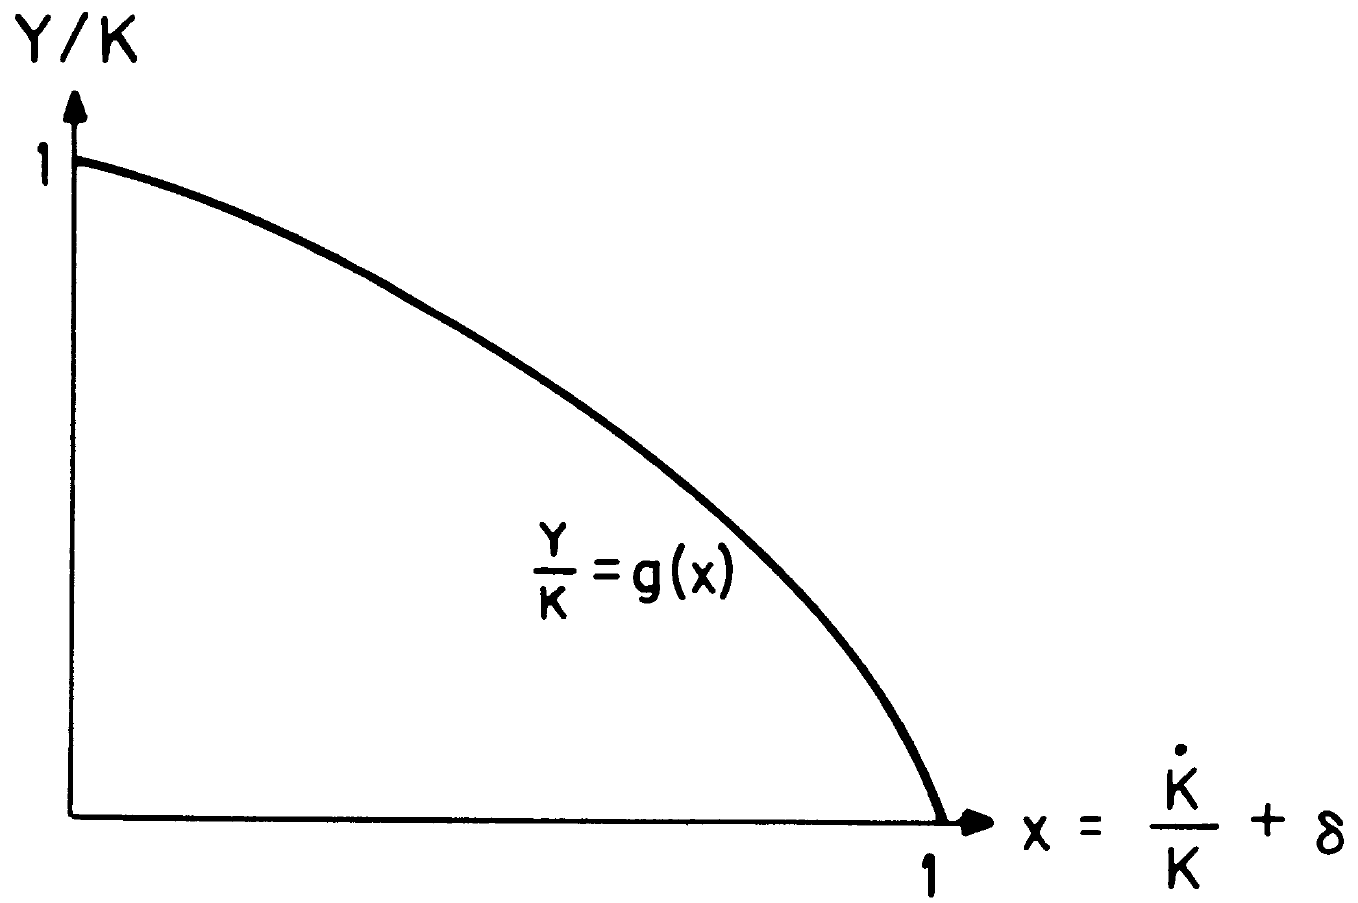
\includegraphics[width=0.8\textwidth]{../output/g.png}
        \centering
    \end{figure}

\end{frame}



\begin{frame}
    \frametitle{Endogenous life phases}
    
    Four phases:
    \begin{wideitemize}
        \item Education: $x = 1$
        \item Work + learning: $0 < x < 1$
        \item Work + no learning: $x = 0$
        \item Retirement: $h = 0$
    \end{wideitemize}

\end{frame}

\begin{frame}
    \frametitle{Endogenous life phases}

    \begin{figure}[t]
        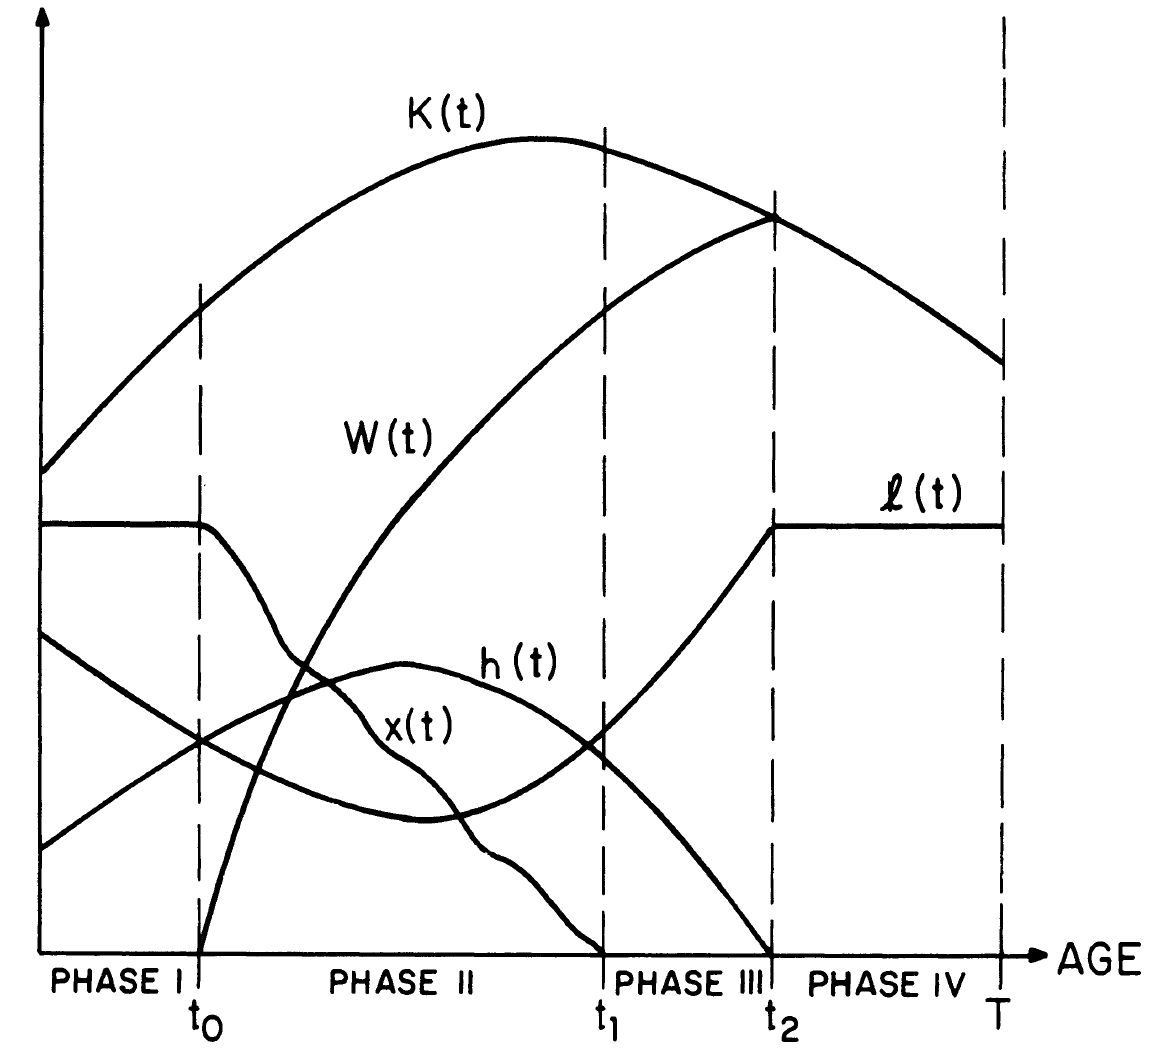
\includegraphics[width=0.6\textwidth]{../output/phases.png}
        \centering
    \end{figure}

\end{frame}



\begin{frame}
    \frametitle{Challenges}

    \begin{wideitemize}
        \item Both shooting method (continuous time model) and backward induction of value function (discrete time model) not working
        \item Possible way forward: discretize labor supply and investment decisions (Keane \& Wolpin 1994)
        \item What is $g(x)$?
        \item What is causing the flattening and steepening of the experience-income profile?
        \begin{wideitemize}
            \item Changes in labor markets; incorporate into the $g(x)$ function?
            \item Changes in monopsony power?
            \item Endogenize changes in the slope of experience-income profile
        \end{wideitemize}
    \end{wideitemize}

\end{frame}



\end{document}
